\documentclass{article}
%%
%% Author: andre
%% 21/05/18
%%

% Preamble
\documentclass[11pt]{article}
\usepackage{basic}
\newcommand{\codigo}[3]{\lstinputlisting[firstline=#1,lastline=#2, caption=Entidade #3]{../scripts/DDL.sql}}

\title{Descrição do sistema Nação Real}
\date{\today}

% Document
\begin{document}
    \maketitle
    \tableofcontents
    \listoffigures
    \lstlistoflistings
    \newpage

    \section{Introdução}
    \label{s-intro}

    Esse sistema destina-se à melhor articulação intra e inter células. Buscamos criar um sistema de comunicação para
    que as ações estejam melhor coordenadas.

    A ideia é que seja um sistema que funcione bem na tela de computador, mas que também seja bem utilizável em celulares.
    Esse documento tem como principal motivação documentar da melhor forma possível o sistema. Da instalação do sistema até
    o estágio final de produção e lançamento.


    \section[DER]{Diagrama Entidade-Relacionamento}
    \label{DER}

    \begin{figure}
        \centering
        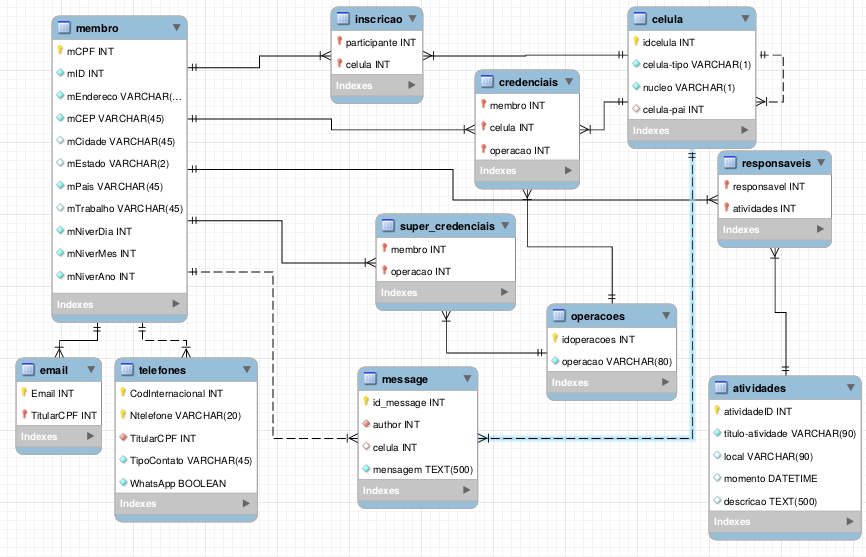
\includegraphics[width=0.85\textwidth]{bd.png}
        \caption{Diagrama que retrata as entidades}
        \label{fig:der}
    \end{figure}

    (Vide figura \ref{fig:der})

    \section[Dependências]{Descrição de dependências}

    Aqui encontra-se uma lista de dependências desse projeto:
    \begin{itemize}
        \item PostgreSQL \dir SGBD \footnote{sistema de gerenciamento de banco de dados}
        responsável pelo armazenamento de dados e transações referentes às operações de
        inserção, leitura, atualização e remoção
        \item psycopg2 \dir biblioteca Pyhton para comunicação com o SGBD
        \item Flask-RESTPlus \dir criação de rotas e requisições REST
        \item Axios \dir parte do front-end, recebem entrada em JSON e trazem os dados de
        forma nítida
        \item Vue \dir ferramenta de front-end, embelezamento
    \end{itemize}
    Abaixo encontram-se instruções de instalação. Tentarei incluir instruções de instalação
    para ambientes Unix/Linux. Caso acharem necessário ou mesmo conveniente, podem colocar
    instruções de instalação em Windows e macOS .

        \subsection{PostgreSQL}
        \subsection{Psycopg2}
        \subsection{Flask-RESTPlus}
        \subsection{Axios}
        \subsection{Vue}

    \section[Descrição]{Entidades e relacionamentos}

        Pra essa sessão, é necessário ter ciência dessa legenda
        \legenda

        \subsection{Membros}
            \codigo{3}{17}{Membros}

            Trata-se da entidade principal do BD. Abaixo estão seus atributos e informações
            relevantes:
            \begin{itemize}
                \item \pk -- \atr{mID} -- inteiro -- identificador serial de tuplas
                \item \atr{mCPF} -- inteiro grande -- escolhido para representar o CPF
                de uma pessoa. Ainda que o CPF possa ser melhor representado por uma string,
                acredito que a indexação seja mais otimizada se processsada com inteiros.
                A principal razão desse campo não ter sido escolhido como chave primária
                é o fato de que a chave primária ser utilizada nas requisições e procedimentos.
                Isso pode tornar-se uma fragilidade de segurança, se considerarmos que, dependendo
                do protocolo utilizado, essa informação pode ficar exposta
                \item \atr{mEndereco} -- string -- endereço do membro. Deve conter, pelo
                menos, o nome da rua, avenida ou o que for.
                \item \atr{mCodPostal} -- string -- representa o código postal de onde a pessoa
                mora. Pode incluir uma funcionalidade de identificação de endereço através do CEP
                \item \atr{mCidade} -- string -- representa a cidade de residência da pessoa
                \item \atr{mEstado} -- string -- representa o estado ou provícia de residência
                da pessoa
                \item \atr{mPais} -- string -- representa o país de residência da pessoa
                \item \atr{mESpecialidade} -- string -- campo importante, onde o usuário
                descreve sua área de formação. Muito útil para pesquisar quem lhe pode ser
                útil pra um determinado fim dentro da organização
                \item \atr{mNasc} -- data -- serve para verificar a idade dos membros.
                Possibilidades de agregar jovens lideranças, e agrupamento por idades
                \item \atr{mPassword} -- string -- devemos nos juntar e verificar condições de senha
                \item \criar O próprio usuário ou um administrador
                \item \ler Todos os usuários que estiverem numa mesma
                célula e os administradores.
                \item \atualizar Somente o próprio usuário
                \item \deletar O próprio usuário ou o administrador.
                \item Reflexão: será que é válido atribuir um campo disciplinar visível apenas por
                admins
            \end{itemize}

        \subsection{Habilidades}

            Tabela representa o múltiplos valores que o campo habilidades e conhecimento podem ter
            \codigo{19}{28}{Habilidades}
            \begin{itemize}
                \item \key  \fk -- \atr{TitularID} -- cahave estrangeira para a entidade Membro
                \item \key -- \atr{habilidade} -- string -- indica a habilidade do membro
                \item \criar O próprio usuário ou o admin
                \item \atualizar Idem
                \item \ler Qualquer usuário.
                \item \deletar Ele mesmo ou o admin
            \end{itemize}

        \subsection{Telefones}

            Tabela reponsável por armazenar os contatos dos membros
            \codigo{30}{42}{Telefones}
            \begin{itemize}
                \item \key -- \atr{CodInternacional} -- inteiro -- Todo o código internacional
                é representado por 1 a 3 dígitos
                \item \key -- \atr{Ntelefone} -- string -- Como não possível saber de todos os
                formatos de números de telefone que poderão ser inseridos, acreditei ser adequado.
                Criar um campo do tipo inteiro limitaria a quantidade de dígitos podendo corromper
                os dados
                \item \key  \fk -- \atr{TitularID} -- cahave estrangeira para a entidade Membro
                \item \atr{Pessoal} -- booleano -- campo destinado a indicar se o número
                indicado é de uso profissional ou pessoal
                \item \atr{WhatsApp} -- booleano -- indica se um perfil de WhatsApp está associado
                à esse número
            \end{itemize}

        \subsection{Email}

            Semelhante à tabela anterior, armazena formas de contato
            \codigo{44}{53}{Email}
            \begin{itemize}
                \item \key \fk -- \atr{TitularID} -- cahave estrangeira para a entidade Membro
                \item \key -- \atr{Email} -- string -- indica o número a ser cadastrado
            \end{itemize}

        \subsection{Célula}

            Tabela responável por armazenar os dados das células.
            \codigo{55}{66}{Célula}
            \begin{itemize}
                \item \pk -- \atr{idcelula} --  chave primária -- número serial
                \item \atr{celula\_tipo} -- inteiro --  representa o alcance da célula. O valor
                desse campo é um inteiro que representa um raio de alcance \begin{enumerate}
                    \item Internacional
                    \item Nacional
                    \item Regional
                    \item Estadual
                    \item Sub-estadual
                    \item Municipal
                    \item Bairro
                \end{enumerate}
                \item \atr{nucleo} -- inteiro -- funciona de uma forma análoga com o campo anterior,
                mas diferentemente do anterior, este campo representa a especialização da célula, ou
                seja, se é uma célula estratégica, organizacional, suporte ...
                \item \fk -- \atr{celula\_pai} -- a ideia de nosso sistema, é que as células possam
                ser criadas natualmemte. Uma célula pode surgir instantâneamente ou a partir de
                alguma outra. Neste caso, a célula tem uma célula-pai
            \end{itemize}

        \subsection{Operações}
        \subsection{Operações}
        \subsection{Células}
        \subsection{Mensagens}
        \subsection{Atividades}
        \subsection{Operações}
        \subsection{Operações}


    \section[Equipe]{Membros da equipe}

    Nossa equipe é formada pelos seguintes membros
    \begin{itemize}
        \item André Luiz Abdalla Silveira
        \item Insira o nome de vocês no arquivo \LaTeX
    \end{itemize}

\end{document}
